\documentclass[]{article}
\usepackage{graphicx}
\usepackage[svgnames]{xcolor} 
\usepackage{fancyhdr}

\usepackage{hyperref}
\usepackage{enumitem}
\usepackage[many]{tcolorbox}
\usepackage{listings }
\usepackage[a4paper, total={6in, 8in}]{geometry}
\usepackage{afterpage}
\usepackage{amssymb}
\usepackage{xepersian}
\usepackage[T1]{fontenc}
\usepackage{tikz}
\usepackage[utf8]{inputenc}
\usepackage{PTSerif} 
\usepackage{seqsplit}

\usepackage{listings}
\usepackage{xcolor}
 
\definecolor{codegreen}{rgb}{0,0.6,0}
\definecolor{codegray}{rgb}{0.5,0.5,0.5}
\definecolor{codepurple}{rgb}{0.58,0,0.82}
\definecolor{backcolour}{rgb}{0.95,0.95,0.92}
 
\NewDocumentCommand{\codeword}{v}{
\texttt{\textcolor{blue}{#1}}
}
\lstset{language=C,keywordstyle={\bfseries \color{blue}}}

\lstdefinestyle{mystyle}{
    backgroundcolor=\color{backcolour},   
    commentstyle=\color{codegreen},
    keywordstyle=\color{magenta},
    numberstyle=\tiny\color{codegray},
    stringstyle=\color{codepurple},
    basicstyle=\ttfamily\normalsize,
    breakatwhitespace=false,         
    breaklines=true,                 
    captionpos=b,                    
    keepspaces=true,                 
    numbers=left,                    
    numbersep=5pt,                  
    showspaces=false,                
    showstringspaces=false,
    showtabs=false,                  
    tabsize=2
}

\lstset{style=mystyle}

\settextfont[BoldFont={XB Zar bold.ttf}]{XB Zar.ttf}




\newcommand{\inputsample}[1]{
    ~\\
    \textbf{ورودی نمونه}
    ~\\
    \begin{tcolorbox}[breakable,boxrule=0pt]
        \begin{latin}
            \large{
                #1
            }
        \end{latin}
    \end{tcolorbox}
}

\newcommand{\outputsample}[1]{
    ~\\
    \textbf{خروجی نمونه}

    \begin{tcolorbox}[breakable,boxrule=0pt]
        \begin{latin}
            \large{
                #1
            }
        \end{latin}
    \end{tcolorbox}
}

%%%%%باکس های طراحی شده برای پاسخ نامه ، میتوانید پاسخ را درون باکس قراردهید
\newtcolorbox[auto counter]{solutionbox}{
freelance,
colback=white,
frame code={},
interior titled code={
  \fill[rounded corners=8pt,orange!30]
    (title.south west) --
    (title.south) -- 
    ([yshift=20pt]title.south) --
    ([yshift=20pt,xshift=4cm]title.south) --
    ([xshift=4cm]title.south) --
    (title.south east) {[sharp corners] --
    ([yshift=-6pt]title.south east) -- 
    ([yshift=-6pt]title.south west) } -- cycle;
  \draw[rounded corners=8pt,gray,line width=1pt]
    (title.west|-frame.south west) --
    (title.south west) --
    (title.south) -- 
    ([yshift=20pt]title.south) --
    ([yshift=20pt,xshift=4cm]title.south) --
    ([xshift=4cm]title.south) --
    (title.south east) --
    (title.east|-frame.south east) --
    cycle;
  \node at ([xshift=2cm,yshift=4pt,anchor=south]title.south) 
    {\Large \textbf{پاسخ}};  
  },
title={\mbox{}},
top=12pt,
fontupper=\sffamily\Large,
oversize=0.5cm,
before={\vskip24pt\par\noindent},
after={\par\vskip12pt}
}
\newtcolorbox[auto counter]{solutionboxC}{
freelance,
colback=white,
frame code={},
interior titled code={
  \fill[rounded corners=8pt,orange!30]
    (title.south west) --
    (title.south) -- 
    ([yshift=20pt]title.south) --
    ([yshift=20pt,xshift=4cm]title.south) --
    ([xshift=4cm]title.south) --
    (title.south east) {[sharp corners] --
    ([yshift=-6pt]title.south east) -- 
    ([yshift=-6pt]title.south west) } -- cycle;
  \draw[rounded corners=8pt,gray,line width=1pt]
    (title.west|-frame.south west) --
    (title.south west) --
    (title.south) -- 
    ([yshift=20pt]title.south) --
    ([yshift=20pt,xshift=4cm]title.south) --
    ([xshift=4cm]title.south) --
    (title.south east) --
    (title.east|-frame.south east) --
    cycle;
  \node at ([xshift=2cm,yshift=4pt,anchor=south]title.south) 
    {\Large \textbf{ پاسخ ادامه}};  
  },
title={\mbox{}},
top=12pt,
fontupper=\sffamily\Large,
oversize=0.5cm,
before={\vskip24pt\par\noindent},
after={\par\vskip12pt}
}

\begin{document}


%%% title pages
\begin{titlepage}
\begin{center}
        
\vspace*{0.7cm}


\includegraphics[width=0.4\textwidth]{sharif1.png}\\
\vspace{0.5cm}
\textbf{ \Huge{\emph درس برنامه‌سازی پیشرفته} }\\
\vspace{0.5cm}
\textbf{ \Large{ تمرین اول} }
\vspace{0.2cm}
       
 
      \large \textbf{دانشکده مهندسی کامپیوتر}\\\vspace{0.2cm}
    \large   دانشگاه صنعتی شریف\\\vspace{0.2cm}
       \large  نیم سال اول 99-00 \\\vspace{0.2cm}
      \noindent\rule[1ex]{\linewidth}{1pt}
    مبحث:\\
    \textbf{{مباحث مقدماتی جاوا}}

    \vspace{0.20cm}

   مهلت ارسال:\\
    \textbf{{25 مهر}}\\
    \textbf{{ساعت 23:59}}

    \vspace{0.15cm}
ویراستار فنی:\\
    \textbf{{پارسا محمدیان و مهدی ابوترابی}}
\end{center}
\end{titlepage}
%%% title pages


%%% header of pages
\newpage
\pagestyle{fancy}
\fancyhf{}
\fancyfoot{}
\cfoot{\thepage}
\chead{مباحث مقدماتی جاوا}
\rhead{
\includegraphics[width=0.1\textwidth]{sharif.png}}
\lhead{تمرین ۱ برنامه‌سازی پیشرفته}
%%% header of pages




 \Large \textbf{\\\\
به موارد زیر توجه کنید:}

\begin{itemize}[label=$\ast$]
\item به‌ازای هر سوال در سامانه‌ی کوئرا، یک بخش جداگانه برای بارگذاری برنامه‌ی شما وجود دارد. برنامه‌ی خود با پسوند .java را در بخش مربوط به هر سوال بارگذاری کنید.
\item ورودی و خروجی شما باید عیناً شبیه به نمونه‌های ورودی و خروجی باشد؛ لذا عبارت‌هایی همچون \lr{"Enter your number"} را قبل از گرفتن ورودی نباید چاپ کنید.
\item پس از ارسال فایل مربوط به هر سوال، سامانه‌ی کوئرا به‌صورت لحظه‌ای برنامه‌ی شما را داوری کرده و نمره‌ی آن سوال را به شما اعلام می‌کند که در صورت کم بودن نمره‌تان، می‌توانید آن را تصحیح کرده و دوباره ارسال کنید.
\item هم‌فکری و هم‌کاری در پاسخ به تمرینات اشکالی ندارد و حتی توصیه نیز می‌شود؛ ولی پاسخ ارسالی شما باید حتما توسط خود شما نوشته شده‌باشد. در صورت هم‌فکری در مورد یک سوال، نام افراد دیگر را به‌صورت کامنت در ابتدای کد هر سوال بنویسید.  این نکته رو در نظر بگیرید که هم‌فکری تنها مربوط به بخش ایده سوال هست نه پیاده‌سازی آن و در صورت محرز شدن تقلب برای فرد خاطی بدون مسامحه \emph{ منفی نمره تمرین}
منظور می‌گردد. 
\item شما می‌توانید تمامی سوالات و ابهامات خود را در سایت کوئرا در بخش مشخص‌شده برای این تمرین بپرسید.
\item به‌ازای هر روز تاخیر در ارسال پاسخ هر سوال، 30 درصد از نمره‌ی کسب‌شده‌ی شما در آن سوال کم می‌شود. به عنوان مثال اگر پاسخ یک سوال را با دو روز تاخیر ارسال کنید، فقط 40 درصد از نمره‌ای که برای آن سوال گرفته‌اید برای شما لحاظ خواهد شد.
\item در کل شما می‌توانید سه روز تاخیر بدون کسر نمره داشته باشد.
\item به ازای هر‌روز ارسال زود‌تر تمرین به شرط کامل بودن، 5\% نمره اضافه به شما تعلق می‌گیرد. سقف تعداد روز‌هایی که  برای این موضوع محاسبه می‌شود چهار است یعنی در صورت ارسال زود‌تر از چهار روز فقط 20\% نمره اضافه به شما تعلق می‌گیرد. 
\item مهلت ارسال تمرین تا ساعت 23:59 روز 25 مهر 1399 است.
\end{itemize}



\newpage
\section{رمز سزار}

 ژولیوس سزار برای اینکه بتواند پیغام های رد و بدل شده بین ارتش را مخفی نگه دارد از یک نوع رمزنگاری استفاده می‌کند.\\
در این رمزنگاری هر حرف الفبا در متن رمزنگاری نشده به حرف بعدی خود در الفبا تبدیل می شود (\lr{z} به \lr{a} تبدیل می شود). متاسفانه ژولیوس سزار مطلع شده که دشمنانش توانستند رمزش را بشکنند برای همین هم تصمیم می گیرد با کمک شما سیستم رمزگذاری جدیدی درست بکند.\\
در این سیستم جدید به جای این که هر حرف یک بار شیفت پیدا کند هر حرف به اندازه جمله دنباله فیبوناچی مکانش در الفبا شیفت پیدا می‌کند یعنی حرف n ام به اندازه \lr{$f(n)$}  (\lr{f}دنباله فیبوناچی است) مقدارش به جلو شیفت پیدا کند.\\
ژولیوس سزار از شما خواهش کرده که براش یک برنامه بنویسید که بتواند با ان متن ها را رمزنگاری و رمزگشایی کند.
\\

\textbf{ورودی}
\\\\
در خط اول ورودی حرف d و یا حرف e می اید. حرف d به این معنا است که باید متن را رمزگشایی کنید و e به این معنا است که باید متن را رمزنگاری کنید
در خط دوم ورودی یک متن متشکل از حروف کوچک الفبای انگلیسی و بدون فاصله به شما داده می‌شود.
\\

\textbf{خروجی}
\\\\
در خروجی باید رمزنگاری شده و یا رمزگشایی شده ی متن داده شده را چاپ کنید. 
\\
\newpage
\inputsample{
e
\\
iamgaiusjuliuscaesar
}

\outputsample{
jbojfqhnrxwwtfozpcvw
}
\inputsample{
d
\\
buvdhssmwpwseg
}

\outputsample{
attackfromleft
}

\newpage


\section{شریف‌نورد}
دانشکده‌ی هوافضا به تازگی از فضاپیمای «شریف نورد» رونمایی کرده است. این فضاپیما دارای n صندلی است که به صورت دوری چیده شده‌اند و به صورت ساعت‌گرد روی آنها شماره‌های ١ تا n نوشته شده است. قرار است در پروازی آزمایشی همه‌ی n دانشجوی دانشکده‌ی هوافضا با این فضاپیما سفر کنند.\\
هرکدام از دانشجویان این دانشکده یک شماره دانشجویی یکتا از ١ تا n دارد. مسئول این پرواز آزمایشی، به هر یک از دانشجویان یک کارت داده که روی هر کدام از آنها یک شماره از ١ تا n نوشته شده است که الزاما یکتا نیست. در هنگام پرواز همه‌ی دانشجویان به ترتیب شماره دانشجویی وارد «شریف نورد» شده و هر کس کارتی که در دستش هست را نگاه می‌کند و به سراغ صندلی با آن شماره می‌رود. اگر آن صندلی خالی بود روی آن می‌نشیند وگرنه c صندلی در جهت ساعت‌گرد جلو می‌رود. اگر صندلی جدید خالی بود می‌نشیند و اگر خالی نبود باز c صندلی در جهت ساعت‌گرد جلو می‌رود. او آن قدر این کار را تکرار می‌کند تا به یک صندلی خالی برسد. سپس آنجا می‌نشیند.\\
\begin{figure}[h]
\centering
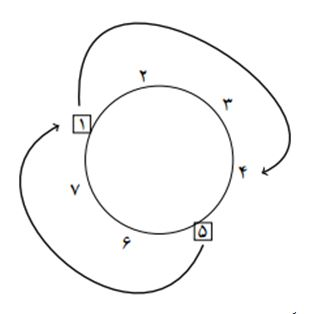
\includegraphics[width=0.5\textwidth]{sharifnavard.JPG}
\end{figure}

مثلاً اگر c برابر ٣ باشد و n برابر ٧ باشد و صندلی ۵ و ١ پر باشند، کسی که بخواهد روی صندلی ۵ بنشیند به جای این که روی ۵ بنشیند روی ۴ مینشیند.\\
مسئول پرواز پس از اینکه همه نشستند برای اینکه به همه نشان دهد باهوش است تصمیم گرفته است بدون این که به صندلی‌ها نگاه کند بگوید هر دانشجویی روی کدام صندلی نشسته است. اما او دید این کار سخت است و آن قدر هم باهوش نیست. لذا از شما درخواست کمک کرده است.\\

\textbf{ورودی}\\\\
در خط اول به ترتیب n و m و c می‌آید. $(m \leq n , 1 \leq c \leq n-1 , m \& n \leq 100)$\\
سپس در خط بعد n عدد می‌آید که عدد i ام، عدد کارت دانشجو با شماره دانشجویی i را مشخص می‌کند. در خط بعد m شماره‌ی دانشجویی از میان n شماره‌ی دانشجویی موجود آمده است که شما باید بگویید هر یک بر روی چه صندلی ای نشسته‌اند (به همان ترتیبی که این m عدد آمده اند.) در این m عدد ممکن است اعداد تکراری نیز وجود داشته باشد.\\

\textbf{خروجی}
\\\\
اگر امکان نشستن همه‌ی افراد وجود نداشت، در خروجی تنها کلمه‌ی Impossible را چاپ کنید. در غیر این صورت شما باید m عدد چاپ کنید که شماره صندلی‌های افرادی است که سوال شده‌اند.\\
\inputsample{
5 4 2\\
5 1 5 2 5\\
4 1 3 5
}
\outputsample{
4 5 2 3
}
\newpage

\inputsample{
6 2 2\\
3 5 1 1 1 1\\
1 2
}
\outputsample{
Impossible
}

\newpage


\section{مسابقه نمکستان}

در شهر نمکستان هر سال قبل از تعطیلات نوروز مسابقه ای برگزار می شود. مسابقه اینگونه است که در ابتدا به هر یک از شرکت کننده ها تعدادی شکلات داده می شود (این تعداد لزوما یکسان نیست)، شرکت کننده ها لیستی تهیه می کنند که نام تعدادی از دوستانشان که در جشن حضور دارند نوشته شده است و شکلات های هر فرد قرار است به صورت مساوی بین نام هایی که در لیست آمده است تقسیم شود(در لیست هر نفر حداقل یک نفر بایستی وجود داشته باشد). به دلیل شیوع ویروس کرونا نمی توان شکلات ها را به صورت اعشاری تقسیم کرد، از این رو اگر تقسیم شکلات ها بین نام های موجود در لیست باقی مانده داشته باشد، باقی مانده نزد صاحب شکلات ها می ماند. مثلا اگر سارا 17 شکلات داشته باشد و بخواهد بین 4 نفر تقسیم کند، 1 شکلات برای خودش باقی می ماند. در پایان این مسابقه برنده کسی است که شکلات بیشتری داشته باشد.\\ 
حال شما برنامه ای بنویسید که پس از گرفتن اسامی شرکت کنندگان، تعداد شکلات های اولیه و لیست تهیه شده توسط هر فرد، لیستی از شرکت کننده ها را به همراه تعداد شکلات هایشان نشان دهد که از بیشتر به کمتر مرتب شده اند.\\
\\
\textbf{ورودی}\\\\
خط 1 : عدد n  که برابر است با تعداد شرکت کنندگان در جشن.\\
خط 2 تا n+1  : در هر خط اسم یکی از شرکت کنندگان.\\
خط n+1  الی آخر : از این خط به بعد ورودی به n  دسته تقسیم می‌شود که هرکدام مطابق زیر است: خط اول نام فردی که قرار است هدیه بدهد. در خط دوم دو عدد می‌آید: عدد اول تعداد شکلات های آن فرد، عدد دوم (k)  تعداد افراد موجود در لیست آن فرد در k  خط بعدی در هر خط نام یکی از افراد موجود در لیست هدیه‌ی آن فرد.\\
می‌توانید فرض کنید نام هر دو نفر از افراد شرکت‌کننده در جشن متمایز است و\\
\begin{latin}
$(2 \leq n \leq 10)$ , 
 $(	1\leq k \leq  n-1 )$\\
\end{latin}
      
\newpage
\textbf{خروجی}\\
\\
در خروجی باید n خط چاپ کنید که در هر ابتدای هر خط نام هر شخص و بعد از آن تعداد شکلات های او آورده شود.( باید ابتدا بیشترین تعداد شکلات یا برنده مسابقه آورده شود یعنی به ترتیب از بیشترین تعداد به کمترین و اگر تعداد شکلات ها برابر بود به ترتیب الفبا مرتب شود)\\

\inputsample{
5\\
dave\\
laura\\
owen\\
vick\\
amr\\
dave\\
200 3\\
laura\\
owen\\
vick\\
owen\\
500 1\\
dave\\
amr\\
150 2\\
vick\\
owen\\
laura\\
0 2\\
amr\\
vick\\
vick\\
0 1\\
owen
}
\outputsample{
dave 502\\
owen 151\\
vick 141\\
laura 66\\
amr 0
}

\newpage
\section{خرید دلار}


رهام در شرکتی آبدارچی شده است و به تازگی اولین حقوق خودش را گرفته است.
 او قصد دارد با پول خود دلار بخرد ولی به دلیل نوسانات بازار ارز نمی‌تواند ساعت مناسبی را برای خرید دلار انتخاب کند.
  هر کدام از دوستان رهام به او ساعتی را پیشنهاد میکنند و رهام هم درصد اعتماد به هر یک از دوستان خود را می‌داند.
رهام این اطلاعات را به این صورت در دفتر خود نوشته است : 
\\
هر سطر شامل یک پیشنهاد است که به صورت \\
\textbf{RECOMMENDER\_NAME/HH:MM:SS/TRUST\_PERCENT}\\
نوشته شده است. (برای مثال 
mamal/04:20:00/80
نشان دهنده یک پیشنهاد از طرف 
mamal
است که ساعت 
04:20:00
را پیشنهاد داده است و رهام 80 درصد به او اطمینان دارد!)

\vspace{1cm}



\textbf{ورودی}
\\ \\
در خط اول ورودی 
n 
که تعداد پیشنهاد‌ها را نشان می‌دهد می‌آید.
سپس در هر کدام از
n
خط بعدی یک پیشنهاد با قالب ذکر شده آمده است. 



\vspace{1cm}

\textbf{خروجی}
\\\\
در خروجی پیشنهادها به ترتیب درصد اعتماد به شکل نزولی و در صورت برابری درصد اعتماد به ترتیب ساعت به شکل صعودی چاپ می‌شوند. برای پیشنهاد‌هایی که ساعت یکسان 
دارند، درصد اعتماد را میانگین درصد اعتماد همه‌ی آن‌ها تا یک رقم اعشار در نظر بگیرید و نام پیشنهاد دهندگان را به ترتیب الفبا با اسپیس از هم جدا کنید.
و در آخر میانگین تمام ساعت‌های پیشنهاد شده (برای محاسبه میانگین فقط از تقسیم اعداد صحیح استفاده کنید کافی است) را چاپ کنید.
 همچنین اگر ساعت ورودی غیر مجاز بود و یا درصد اعتماد در بازه 1 تا 100 نبود آن پیشنهاد حذف می‌شود و در خروجی هم نمایش داده نمی‌شود.
\\


\inputsample{
4
\\
pouya/12:43:32/70
\\
bardia/05:23:61/12
\\
hooman/09:00:00/91
\\
kahbod/12:43:32/2
}

\outputsample{
hooman/09:00:00/91
\\
kahbod pouya/12:43:32/36
\\
11:29:01
}

\newpage
\section{شبکه اجتماعی x}


x به تازگی یک شبکه اجتماعی مانند اینستاگرام تاسیس کرده است که ویژگی عجیبی دارد. در این شبکه هر کس چند دنبال شونده (0 تا \lr{n}) دارد و هرکس می‌تو‌‌‌اند فقط یک نفر را دنبال کند که آن یک نفر خودش هم می‌تواند باشد(هم دنبال کننده خودش باشد هم دنبال شونده خودش) . این شبکه هر دفعه به یک سری از مشترکینش جایزه میدهد. x  بزرگ ترین گروهی از افراد را که شرایط زیر را دارند میخواهد تا به آنها جایزه دهد و هرکس این شرایط را نداشته باشد جزو دنبال کننده های افراد دیگر به حساب نخواهد امد(مثال تصویری را در آخر سوال ببینید) :
\begin{itemize}
\item
 هر نفر در آن لیست حتما توسط یک فرد دیگر در همان لیست دنبال می‌شود.(آن یک نفر نیز حتما میتواند خودش باشد- حالت فالو کردن خودش)
\item
هرکس تعداد دنبال کننده هایش دقیقا 1 نفر است.
\end{itemize}
این لیست را به x بدهید.\\\\
\textbf{ورودی}\\\\
در خط اول عدد n می آید که بیانگر تعداد افراد است و در خط بعدی n عدد می‌آید که عدد i ام برابر شماره فرد فالو شده توسط i ام است.\\

\textbf{خروجی}\\\\
در خط اول اندازه‌ی بزرگترین زیر مجموعه و در خط بعدی افراد در آن زیر مجموعه‌ را خروجی دهید.

\newpage
\inputsample{
6\\
2 2 4 4 6 6
}
\outputsample{
3\\
2 4 6
}
\vspace{1cm}
\textbf{توضیحات بیشتر}\\\\
در این مثال 6 نفر وجود دارند که به ترتیب نفر اول  شماره 2 - نفر دوم شماره 2 - نفر سوم و چهارم شماره 4 - نفر پنجم و ششم شماره 6 را فالو کرده اند. یعنی نفرات 1و 3و 5 را هیچکس فالو نکرده است.به همین دلیل در زیرمجموعه ما قرار نمیگیرند و حذف میشوند. حال 3 نفر 2و4و6 باقی میمانند که دو شرط داده شده را دارند.
\begin{figure}[h]
\centering
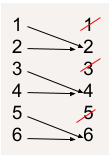
\includegraphics[width=0.2\textwidth]{social1.png}
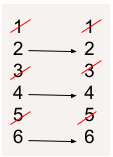
\includegraphics[width=0.2\textwidth]{social2.png}
\end{figure}

\end{document}









